\documentclass[a4paper]{article}

\usepackage{tikz}
\usetikzlibrary{positioning}

\title{PaperTrader Protocol Specification}
\author{altffour}
\date{\today}

\begin{document}
\maketitle
\tableofcontents
\newpage

\section{Introduction}
This is the document for the specification of PaperTrader. PaperTrader is an
application for 'fake' trading assets, to practice investing. The document
contains explainations on how to implement the papertrader application. It 
should be noted that the document isn't `production-ready' until this sentence 
is removed. The document will go over the roles of the master server, and the
worker servers, how they interact with eachother and the communication protocol,
and finally, suggestions on server side implementations.

\section{Overview}
This section contains the required terminology and modelling of the PaperTrader
infrastructure.

\subsection{Terminology}

\subsubsection{Inner World}
This is Master server, and all worker servers. This should be kept under high
lockdown. Meaning, critical data should be kept secure.

\subsubsection{Outer World}
This is the frontend, including the desktop cleint, mobile client, or the
website client. The data here is controlled by the authorization of the account.

\subsubsection{Critical Data}
Cirtical Data are all data types that shouldn't be tampered with without
authorization. For example, accounts, personal information, messages, and in
this context user's portfolios.

\subsubsection{User/Client}
In this context it is the frontend, which is either the desktop client,
mobile client, or the website client.

\subsubsection{User/Client Data}
This is the data of the user. The meaning depends on the specific conext. It
could mean the personal information, credentials, etc. Most of the time it means
data that is attached to a data transfer to identify client (IP?).

\subsubsection{Master Server}
This is the main server that MUST be run when deploying the application.
Contains critical data, it would only interact to the outside world by the
worker servers.

\subsubsection{Worker Servers}
These are servers that contact the outer world. Worker Servers will
interact with the Master Server acting like a `cache' servers. Data should be 
routed through worker servers to the master server. The main job for worker 
server is to add timestamps onto commands sent from the user. The data sent to
the main server must contain the data of the client/user. There MUST be ATLEAST
one instance running to have a functional infrastructure.

\subsubsection{User Accounts}
This is the account that abstractly is a the data structure that contains
information about hte user and their account.

\subsection{Infrastructure Model}
A fully deployed infrastructure cotains \emph{ONE} master server, 
\emph{ATLEAST} one worker server, theoretically across the world to maintain 
speed and reliabilty. An overview diagram of the infrastructure: \newline

\begin{center}
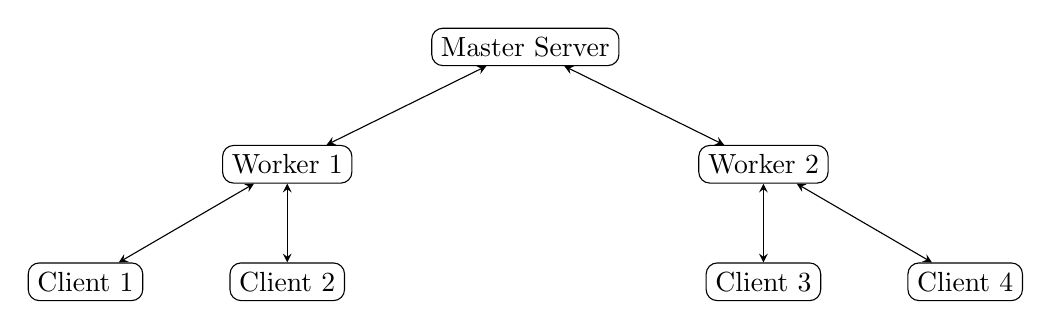
\begin{tikzpicture}[>=stealth,every node/.style={shape=rectangle,draw,rounded 
	corners}]
    % create the nodes
    \node (master) {Master Server};
    \node (worker1) [below left=of master]{Worker 1};
    \node (worker2) [below right=of master]{Worker 2};
	\node (client1) [below left=of worker1]{Client 1};
	\node (client12) [below =of worker1]{Client 2};
	\node (client2) [below =of worker2]{Client 3};
	\node (client22) [below right=of worker2]{Client 4};
    % connect the nodes
    \draw[<->] (master) -- (worker1);
    \draw[<->] (master) -- (worker2);
    \draw[<->] (worker1) -- (client1);
    \draw[<->] (worker2) -- (client2);
    \draw[<->] (worker1) -- (client12);
    \draw[<->] (worker2) -- (client22);
\end{tikzpicture} 
\end{center}

\newpage
\subsubsection{Master Server Infrastructure Model}
The master server is contains critical data. It can be defined into modules as
demonstrated in the following diagram: \newline

\begin{center}
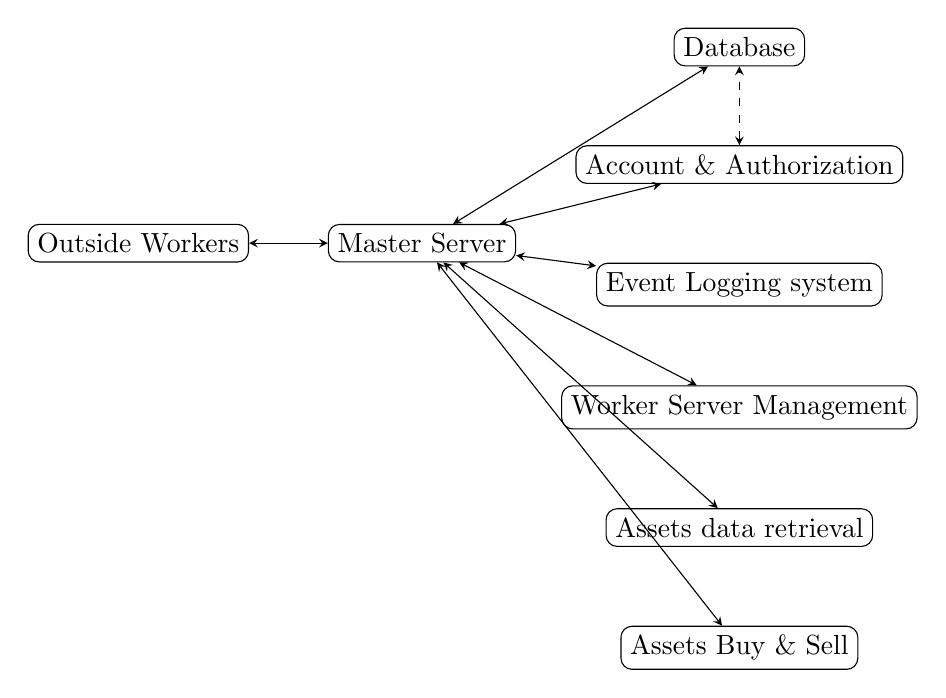
\begin{tikzpicture}[>=stealth,every node/.style={shape=rectangle,draw,rounded
	corners}]
	% create the nodes.
	\node (master) {Master Server};
	\node (db) [above right=2cm and 2cm of master]{Database};
	\node (acc) [below=of db]{Account \& Authorization};
	\node (log) [below=of acc]{Event Logging system};
	\node (worker) [below=of log]{Worker Server Management};
	\node (asset) [below=of worker]{Assets data retrieval};
	\node (assettrans) [below=of asset]{Assets Buy \& Sell};
	\node (outsideworkers) [left=of master] {Outside Workers};

    % connect the nodes
    \draw[<->] (outsideworkers) -- (master);
    \draw[<->] (master) -- (db);
    \draw[<->] (master) -- (acc);
    \draw[<->, dashed] (acc) -- (db);
    \draw[<->] (master) -- (log);
    \draw[<->] (master) -- (worker);
    \draw[<->] (master) -- (asset);
    \draw[<->] (master) -- (assettrans);
\end{tikzpicture}
\end{center}

\end{document}
